\graphicspath{{./Einfuehrung/eps/}}

\cleardoublepage
%%%%%%%%%%%%%%%%%%%%%%%%%%%%%%%%%%%%%%%%%%%%%%%%%%%%%%%%%%%%%%%%%%%%%%%%%%%%%%%%%%%%%%%%%%%%%%%%%%%%%%%%%%%%%%%%%%%%%%%%%%%%

\chapter{Einf\"{u}hrung}

%%%%%%%%%%%%%%%%%%%%%%%%%%%%%%%%%%%%%%%%%%%%%%%%%%%%%%%%%%%%%%%%%%%%%%%%%%%%%%%%%%%%%%%%%%%%%%%%%%%%%%%%%%%%%%%%%%%%%%%%%%%%

\section{Begriffserl\"{a}uterungen}

%%%%%%%%%%%%%%%%%%%%%%%%%%%%%%%%%%%%%%%%%%%%%%%%%%%%%%%%%%%%%%%%%%%%%%%%%%%%%%%%%%%%%%%%%%%%%%%%%%%%%%%%%%%%%%%%%%%%%%%%%%%%
Zum besseren Verst\"{a}ndnis des Benutzerhandbuchs seien vorab einige immer wiederkehrende Begriffe n\"{a}her erl\"{a}utert.
\begin{description}
   \item[Programmsystem~\wspwin{}:]
      Das Programmsystem \wspwin{} umfa{\ss}t das komplette Spiegellinienprogramm inklusive Windows-Oberfl\"{a}che \wspwin{},
      Berechnungsprogramm WSPR (Prof. Knauf) oder BCE-WSP (Prof. Pasche),
      Plotprogramm BCE-PRO Plotter sowie s\"{a}mtliche Zusatzmodule und Unterprogramme.
   \item[Windows-Oberfl\"{a}che~\wspwin{}:]
      Die Windows-Oberfl\"{a}che \wspwin{} im engeren Sinne bezeichnet die Masken, Fenster und Dialoge gestaltet in Look and
      Feel von MS-Windows, \"{u}ber die die geometrischen und hydraulischen Daten f\"{u}r das Berechnungsprogramm WSPR eingegeben
      werden. Die Oberfl\"{a}che wurde von der Bj\"{o}rnsen Beratende Ingenieure GmbH, Koblenz entwickelt.
   \item[Berechnungsprogramm WSPR (entspr. WSPLWA, WSP97P, HYDRA-WSP):]
      Das \\ Berechnungsprogramm WSPR ist ein separates Programm, das aus der
      Windows-Oberfl\"{a}che heraus aufgerufen wird. WSPR kann auch ohne die Windows-Oberfl\"{a}che
      gestartet werden, allerdings sind dann aufwendige Formatanweisungen bei der Dateneingabe einzuhalten. \newline
      Die Bezeichnungen WSPR, WSPLWA, WSP97P (bei Programmen aus anderen Jahren kann die 97 entsprechend ersetzt werden)
      sind identisch. Der Name WSPR wurde gew\"{a}hlt, um anstatt der ehemals unterschiedlichen Bezeichnungen einen eindeutigen
      Namen zu erhalten. Im Landesumweltamt Nordrhein-Westfahlen (ehemals LWA-NRW) ist das Berechnungsprogramm bereits seit
      1968 im Einsatz, soda{\ss} sich teilweise auch der Name WSPLWA eingeb\"{u}rgert hat. WSPR ist Bestandteil des Programmpaketes
      HYDRA, das neben dem eigentlichen Wasserspiegellagenprogramm (HYDRA-WSP) weitere Programme f\"{u}r hydraulische
      Bemessungen im Bereich Wasserbau, Verkehrsbau und Stadtentw\"{a}sserung umfa{\ss}t. Das Berechnungsprogramm wurde vom
      Programmservice Wasserwirtschaft Knauf, Seeheim-Jugenheim entwickelt.
   \item[Projekt:]
      Ein Projekt stellt ein vom Benutzer definiertes Verzeichnis dar, in dem s\"{a}mtliche Verkn\"{u}pfungs-, Profil- und
      Ergebnisdateien abgelegt werden, die in einem inhaltlichen Zusammenhang zueinander stehen,
      z.B. \datei{C:\textbackslash projekte\textbackslash fulda}.
      Beim Neuanlegen eines Projektes werden in diesem Verzeichnis programmintern automatisch die beiden Unterverzeichnisse
      \datei{...\textbackslash dath} und \datei{...\textbackslash prof} angelegt, wobei das Steuerprogramm im weiteren
      Arbeitsverlauf s\"{a}mtliche Berechnungsergebnisse im Unterverzeichnis \datei{...\textbackslash dath} und alle \"{u}brigen
      Dateien im Unterverzeichnis \datei{...\textbackslash prof} ablegt.
      Zu jedem Projekt wird im Unterverzeichnis \datei{...\textbackslash prof} eine Datei \datei{profproj.txt} angelegt,
      in der s\"{a}mtliche Profile eines Projektes mit ihren Schl\"{u}sseldaten, sowie die Zustandsdateien, die sich auf diese
      Profile beziehen, referenziert sind. Hier\"{u}ber wird w\"{a}hrend des Programmablaufs gepr\"{u}ft, ob Schl\"{u}sseldaten doppelt
      vergeben wurden.
\end{description}
\begin{hinweis}
   Bitte vermeiden Sie es, im Projektverzeichnis andere als \"{u}ber \wspwin{} referenzierte Dateien abzulegen.
\end{hinweis}
\begin{description}
   \item[Zustandsdatei, Vernetzungsdatei:]
      Eine Vernetzungsdatei (Ver\-kn\"{u}p\-fungs\-da\-tei, Zu\-stands\-da\-tei) stellt eine Indexdatei
      dar, in der alle Profile, die zu einem geometrischen Zustand (z.B. Planung, Bauphase etc.) geh\"{o}ren, \"{u}ber
      Schl\"{u}sselw\"{o}rter zusammengefa{\ss}t sind. In der Vernetzungsdatei sind keine Profildaten, sondern lediglich Zeiger auf die
      entsprechenden Profildateien abgelegt. Die Reihenfolge, in der die Profile entlang des Gew\"{a}ssers auftreten und in der
      sie w\"{a}hrend einer Spiegellinienberechnung abgearbeitet werden, sowie der Abstand zwischen den Profilen im Flu{\ss}schlauch
      bzw. auf den Vorl\"{a}ndern werden in der Strangtabelle als Teil der Vernetzungsdatei festgelegt. Die Zuordnung erfolgt
      \"{u}ber die drei Parameter Gew\"{a}ssername, Zustand und Datum, die vom Benutzer zu definieren sind. Innerhalb eines
      Projektes k\"{o}nnen mehrere Vernetzungsdateien definiert werden, die Referenzen auf die gleichen, aber auch auf
      unterschiedliche Profildateien beinhalten k\"{o}nnen.
      \\ Dateiname: z.B. \datei{fu000001.str}
   \item[Strangtabelle:]
      Die Aufeinanderfolge der Profile entlang des Gew\"{a}ssers ist durch die Strangtabelle definiert. Sie entspricht auch der
      Reihenfolge der Abarbeitung bei der Spiegellinienberechnung. Dar\"{u}ber hinaus wird hier der Abstand zwischen den
      Profilen im Flu{\ss}schlauch und auf den Vorl\"{a}ndern festgelegt. Die Strangtabelle wird standardm\"{a}{\ss}ig mit einer sortierten
      Liste der Stationswerte vorbesetzt. Die Profilabst\"{a}nde werden aus den vom Benutzer beim Neuanlegen oder Konvertieren
      von Profilen eingegebenen Stationswerten zun\"{a}chst f\"{u}r die Vorl\"{a}nder und den Flu{\ss}-schlauch einheitlich besetzt.
      Eine Editierung der Strangtabelle durch den Nutzer ist nur dann erforderlich, wenn oder unterschiedliche
      Profilabst\"{a}nde f\"{u}r Vorl\"{a}nder und Flu{\ss}schlauch (z.B. bei stark m\"{a}andrierenden Gew\"{a}ssern) vorliegen.
      Unter Umst\"{a}nden kann es erforderlich sein, nach der automatischen Sortierung verzweigter Systeme die Abst\"{a}nde zu
      pr\"{u}fen und zu korrigieren. Bei einer umgekehrten Stationierung ist ein entsprechender Schalter vor Einf\"{u}gen der
      Profile zu aktivieren, damit die Stationierung absteigend erfolgt.
   \item[Profiltabelle:]
      Neben der Strangtabelle besteht die Vernetzungsdatei aus der Profiltabelle (einer Liste mit s\"{a}mtlichen zum Zustand
      geh\"{o}renden Profilen). Hinterlegt ist der Profilschl\"{u}ssel und der zugeh\"{o}rige Profildateiname.
   \item[Abflu{\ss}datei:]
      F\"{u}r eine Spiegellinienberechnung ist als Randbedingung der Durchflu{\ss} an einzelnen Stationen zu definieren. Hierzu
      dient die Abflu{\ss}datei. Eine Abflu{\ss}datei ist jeweils einer Vernetzungsdatei zugeordnet, so da{\ss} f\"{u}r jede
      Vernetzungsdatei stets eine Abflu{\ss}datei zu definieren ist. In dieser Datei wird der Abflu{\ss} profilbezogen festgelegt.
      Dabei m\"{u}ssen jedoch nur diejenigen Profile eine Abflu{\ss}definition erfahren, an denen eine Abflu{\ss}\"{a}nderung im Vergleich
      zum vorherigen Profil stattfindet. Innerhalb einer Abflu{\ss}datei besteht die M\"{o}glichkeit der Differenzierung
      verschiedener Abflu{\ss}ereignisse (z.B. HQ1, HQ2, HQ100). Bei der Spiegellinienberechnung kann der Anwender dann den
      gew\"{u}nschten Abflu{\ss}zustand ausw\"{a}hlen. Dateiname: z.B. \datei{fu000001.qwt}
   \item[Wasserspiegelfixierungen:]
      F\"{u}r jedes Abflu{\ss}ereignis k\"{o}nnen an den vorhandenen Stationen gemessene Wasserspiegelh\"{o}hen eingegeben werden. Die
      Wasserspiegelfixierungen werden im Rahmen der Berechnung automatisch in die L\"{a}ngsschnitte eingetragen.
      \\ Dateiname: z.B. \datei{fu000001.wst}
   \item[Verlustdatei:]
      In der Einzelverlustdatei k\"{o}nnen \"{o}rtlich auftretende Flie{\ss}verluste, wie sie z.B. an Rohreinl\"{a}ufen, Rechen,
      Gerinneverzweigungen etc. auftreten, auf das einzelne Profil bezogen, definiert werden. Die Ablage der Einzelverluste
      getrennt von den Profildaten in einer eigenst\"{a}ndigen Datei bietet dem Anwender mehr Flexibilit\"{a}t in der Definition
      dieser Verluste. Es sind die Verlusttypen Einlauf, Kr\"{u}mmer, Rechen und Zusatzverlust definierbar, wobei an einer
      Station maximal 5~Verluste m\"{o}glich sind, die programmintern sp\"{a}ter addiert werden.
      \\ Dateiname: z.B. \datei{fu000001.psi}
   \item[Profildatei:]
      Die Profildatei enth\"{a}lt s\"{a}mtliche geometrischen und hydraulischen Daten, die ein Querprofil beschreiben. Ihr Inhalt
      variiert in Abh\"{a}ngigkeit vom Profiltyp (z.B. Normalprofil, Br\"{u}ckenprofil, Wehrprofil). Die Profildatei setzt sich aus
      dem Profilschl\"{u}ssel (Gew\"{a}ssername, Stations-km, Profilzustand, Verzweigungs- und Profilkennung), \"{u}ber den das Profil
      eindeutig referenziert ist, und sogenannten Datenblocktypen (z.B. Gel\"{a}ndeh\"{o}he, Rauheit, Lage der Trennfl\"{a}chen etc.)
      mit den zugeh\"{o}rigen Werten zusammen. Die Profildatei ist sowohl alphanumerisch wie auch grafisch-interaktiv editierbar.
      \\ Dateiname: z.B. \datei{fu000001.prf}
   \item[Datenblocktypen:]
      Als Datenblocktypen werden geometrische und hydraulische Parameter bezeichnet, durch die eine Profildatei
      charakterisiert wird. Im Kapitel zum Grafikeditor sind s\"{a}mtliche in \wspwin{} verf\"{u}gbaren Datenblocktypen tabellarisch
      aufgelistet. Nach dem Anlegen eines Datenblocktyps oder Datensatzes sind die entsprechenden Wertepaare einzugeben
      (z.B. Gel\"{a}ndeh\"{o}he in $\mathrm{[NN+m]}$, Rauheit im $\mathrm{[m]}$ oder $\mathrm{[m^{1/3}/s]}$ usw.).
   \item[Berechnungsvarianten:]
      Beim Aufruf des Spiegellinienprogramms erfolgt die Abfrage der notwendigen Steuerbefehle f\"{u}r die Programmausf\"{u}hrung.
      Diese werden in einer separaten Datei gespeichert. Damit hat der Benutzer die M\"{o}glichkeit, mehrere Steuerdateien
      zun\"{a}chst zu erstellen, (eventuell auch wieder zu \"{a}ndern oder zu l\"{o}schen) und anschlie{\ss}end die
      Spiegellinienberechnung f\"{u}r diese Steuerdateien im Batchbetrieb auszuf\"{u}hren. Einen \"{U}berblick \"{u}ber die einzelnen Berechnungsvarianten eines
      jeweiligen Zustands gibt die Berechnungsvariantenverkn\"{u}pfungsdatei. F\"{u}r jede Zustandsdatei wird eine solche Datei
      automatisch angelegt. F\"{u}r die eigentliche Spiegellinienberechnung besteht dann die M\"{o}glichkeit mehrere der
      Berechnungsvarianten (auch aus verschiedenen Verkn\"{u}pfungsdateien) auszuw\"{a}hlen und in einem Schritt im Stapelbetrieb
      berechnen zu lassen.
      \\ Dateiname Berechnungsvariantenverkn\"{u}pfung:  z.B. \datei{fu000001.ber}
      \\ Dateiname Berechnungsvarianten: z.B. \datei{fu000001.001}
\end{description}


%%%%%%%%%%%%%%%%%%%%%%%%%%%%%%%%%%%%%%%%%%%%%%%%%%%%%%%%%%%%%%%%%%%%%%%%%%%%%%%%%%%%%%%%%%%%%%%%%%%%%%%%%%%%%%%%%%%%%%%%%%%%
\section{Verwendete Formelzeichen und Indices}
%%%%%%%%%%%%%%%%%%%%%%%%%%%%%%%%%%%%%%%%%%%%%%%%%%%%%%%%%%%%%%%%%%%%%%%%%%%%%%%%%%%%%%%%%%%%%%%%%%%%%%%%%%%%%%%%%%%%%%%%%%%%

\input{Einfuehrung/tab/Formelzeichen.tab}
\begin{tabular}{lll}
   \textbf{Indices:} \hspace{1cm}   &  $F$            &  Flu{\ss}schlauch \\
                                    &  $L$            &  linkes Vorland \\
                                    &  $R$            &  rechtes Vorland \\
                                    &  $T$            &  Trennfl\"{a}che \\
                                    &  $\mathit{li}$  &  links \\
                                    &  $\mathit{re}$  &  rechts \\
                                    &  $m$            &  arithmetischer Mittelwert \\
                                    &  $i$            &  Profil $(i)$ \\
                                    &  $i-1$          &  Profil $(i-1)$ (flu{\ss}ab) \\
                                    &  $i+1$          &  Profil $(i+1)$ (flu{\ss}auf) \\
                                    &  $j$            &  Teilabflu{\ss}querschnitt \\
                                    &  $\mathit{II}$  &  Bereich~II \\
                                    &  $\mathit{III}$ &  Bereich~III \\
                                    &  $\mathit{cal}$ &  Rechenwert\\
                                    &  $\mathit{ges}$ &  gesamt\\
\end{tabular}


%%%%%%%%%%%%%%%%%%%%%%%%%%%%%%%%%%%%%%%%%%%%%%%%%%%%%%%%%%%%%%%%%%%%%%%%%%%%%%%%%%%%%%%%%%%%%%%%%%%%%%%%%%%%%%%%%%%%%%%%%%%%
\section{Voraussetzungen}
%%%%%%%%%%%%%%%%%%%%%%%%%%%%%%%%%%%%%%%%%%%%%%%%%%%%%%%%%%%%%%%%%%%%%%%%%%%%%%%%%%%%%%%%%%%%%%%%%%%%%%%%%%%%%%%%%%%%%%%%%%%%

\subsection{Allgemeine Grundlagen}
\label{Einfuehrung Subsec AllgemeineGrundlagen}

Das Programmsystem \wspwin{} dient zur Berechnung der Wasserspiegellagen bei sta\-tio\-n\"{a}r ungleichf\"{o}rmigem Abflu{\ss} in
nat\"{u}rlichen Gerinnen mit Sonderbauwerken. Mit Hilfe des Rechenprogramms k\"{o}nnen folgende Probleme behandelt werden:
\begin{itemize}
   \item Abflu{\ss}vorg\"{a}nge in gegliederten Flu{\ss}querschnitten
   \item Str\"{o}mender und schie{\ss}ender Abflu{\ss}
   \item Einengungen und diskontinuierliche Erweiterungen der Flie{\ss}querschnitte, Pfeilerstau
   \item Berechnung von Durchl\"{a}ssen und Drosselstrecken mit oder ohne \"{U}berflutung
   \item Berechnung von vollkommenen und unvollkommenen \"{U}berf\"{a}llen sowie Streichwehren
   \item Berechnung von Grenztiefen und Normalwassertiefen
   \item Eichung von Rauheitsbeiwerten
   \item Berechnung der Wassermengenaufteilung bei Stromverzweigungen
   \item Berechnung von Abflu{\ss}kurven (Q-H-Kurven) f\"{u}r gegliederte Querschnitte oder Sonderprofile
   \item Berechnung von Mehrfeldbr\"{u}cken
   \item Berechnung der Retentionsparameter nach \autor{Kalinin-Miljukov}
   \item Ber\"{u}cksichtigung von durchstr\"{o}mtem Bewuchs mit Interaktion der Bewuchselemente
\end{itemize}
F\"{u}r die Berechnung einer Gerinnestrecke werden die folgenden Unterlagen bzw. Daten ben\"{o}tigt:
\begin{itemize}
   \item Lageplan und Querprofile der Gerinnestrecke
   \item Angaben \"{u}ber die Rauheitsbeiwerte oder Me{\ss}werte f\"{u}r Wasserstand und Abflu{\ss}
   \item Angaben \"{u}ber Einbauten bzw. Sonderprofile, Bewuchs
   \item Bemessungsabfl\"{u}sse
   \item Hydraulische Steuerparameter (Anfangswasserstand oder Angaben zu dessen Berechnung)
\end{itemize}
Das Rechenprogramm bereitet die Eingabedaten auf, pr\"{u}ft sie auf Vollst\"{a}ndigkeit und Plausibilit\"{a}t, berechnet die
Wasserspiegelh\"{o}hen (ggf. die Rauheitsbeiwerte) und druckt die Eingabedaten, die berechneten geometrischen und
hydraulischen Kennwerte der Querprofile und die Wasserspiegelh\"{o}hen aus.

Ein offener Gerinnequerschnitt kann in h\"{o}chstens drei Teilabflu{\ss}fl\"{a}chen untergliedert werden, wie z.B. in linkes Vorland,
Flu{\ss}schlauch und rechtes Vorland. Die Abgrenzung der Teilfl\"{a}chen kann bei der Dateneingabe beliebig durch Kennzeichnung
der Grenzpunkte vorgegeben werden. Die Aufteilung des Gesamtabflusses in die einzelnen Teilstr\"{o}me ergibt sich aus dem
Verh\"{a}ltnis der hydraulischen Widerstandskr\"{a}fte in den Teilabflu{\ss}fl\"{a}chen zur Gesamtwiderstandskraft. Die hydraulische
Widerstandskraft h\"{a}ngt von den Rauheitsbeiwerten, den hydraulischen Radien, den Querschnittsgr\"{o}{\ss}en und den L\"{a}ngen der
Flie{\ss}wege ab. Die Flie{\ss}wege (Profilabst\"{a}nde) k\"{o}nnen in den Vorl\"{a}ndern und im Flu{\ss}schlauch unterschiedlich sein.

Bei Mehrfeldbr\"{u}cken ist die Anzahl der durchstr\"{o}mten Br\"{u}cken\"{o}ffnungen unbegrenzt. Die einzelnen Flut\"{o}ffnungen k\"{o}nnen durch
beliebige offene oder geschlossene Sonder-profile beschrieben werden. Die Berechnung der Wandreibungsverluste kann
wahlweise mit der Flie{\ss}formel von \autor{Manning-Strickler} oder dem Flie{\ss}gesetz von \autor{Prandtl-Colebrook}
durchgef\"{u}hrt werden.

\subsubsection{Festlegung zur Auftragung von Querprofilen}
Der allgemein \"{u}blichen Konvention entsprechend, erfolgt die Zuordnung von links nach rechts in Flie{\ss}richtung. Zur
Vermeidung von falschen Zuordnungen sollten die Querprofile grunds\"{a}tzlich in Flie{\ss}richtung gesehen aufgetragen werden. Das
linke Vorland liegt in Flie{\ss}richtung gesehen links.

\subsubsection{Festlegung zur Reihenfolge der Profildaten}
Die Reihenfolge der Profileingabe ist dagegen durch die Berechnungsrichtung entgegen der Flie{\ss}richtung festgelegt, d.h.
die Dateneingabe beginnt grunds\"{a}tzlich im unterwasserseitigen Anfangsprofil. Dies gilt auch f\"{u}r den schie{\ss}enden
Abflu{\ss}bereich. Die Stationierungsrichtung ist nicht festgelegt. Es wird jedoch empfohlen, im Sinne des
Gew\"{a}sserverzeichnisses NRW grunds\"{a}tzlich von der M\"{u}ndung in Richtung Quelle zu stationieren.

\subsubsection{Festlegung von EDV-bedingten H\"{o}chstwerten}

Datenverarbeitungsbedingt ist die Anzahl der einzugebenden Daten pro Querprofil und Gerinneabschnitt (Zustand) begrenzt. Pro Zustand k�nnen zur Zeit 3000 Querprofile eingegeben werden, l�ngere Berechnungsstrecken sind in Abschnitte aufzuteilen, die bis zu 3000 Querprofile umfassen k�nnen.
Ein Querschnitt kann in h�chstens 3 Teilabflu�fl�chen untergliedert werden, wie z.B. in linkes Vorland, Flussschlauch und rechtes Vorland. Die gr��tm�gliche Anzahl der je Querprofil einzugebenden Profilpunkte ist auf 1000 begrenzt.

Unabh�ngig von den in der Programmoberfl�che WspWin festgesetzten Maximalwerten k�nnen die Grenzwerte f�r den jeweilig benutzten Rechenkern abweichen. Die jeweils g�ltigen Grenzwerte sind der Dokumentation des Rechenkerns zu entnehmen.

Der logische Zusammenhang eines Stromverzweigungsnetzes ist in den entsprechenden Dialogmasken beim Editieren der
Steuerdaten f\"{u}r die Berechnung einzugeben. Jede Teilstrecke mu{\ss} mindestens einen Zuflu{\ss} und einen Abflu{\ss} aufweisen. Als
Startwerte f\"{u}r die Abflu{\ss}aufteilung k\"{o}nnen die Teilabfl\"{u}sse in Prozent von der dem jeweiligen Verzweigungspunkt
zuflie{\ss}enden Wassermenge angegeben werden. Die Anzahl der Flu{\ss}teilstrecken einer Verzweigung ist auf 20 pro
Rechenabschnitt begrenzt. Art und Anzahl der Querprofile einer Flu{\ss}teilstrecke sind beliebig, lediglich die Gesamtanzahl der Profile eines Abschnittes darf 3000 nicht \"{u}bersteigen. Jeder Knoten kann maximal 2 Zufl�sse und zwei Abfl�sse haben. Bei mehr als zwei Abzweigungen ist ein fiktiver Strang zum Aufbau der Netzlogik erforderlich.

Die Profileingabe erfolgt auch bei verzweigten Gerinnestrecken in Richtung der Berechnung des str\"{o}menden Abflu{\ss}zustandes,
d.h. grunds\"{a}tzlich entgegengesetzt zur Flie{\ss}richtung.

\subsection{Theoretische Grundlagen}
\label{Einfuehrung Subsec TheoretischeGrundlagen} Das grundlegende Verfahren zur Berechnung des Wasserspiegels bei
station\"{a}r ungleichf\"{o}r\-migem Abflu{\ss} in nichtprismatischen Gerinnen besteht in einer von Profil zu Profil fortschreitenden
Berechnung diskreter Wasserspiegelh\"{o}hen, wobei der Energieh\"{o}\-henvergleich nach \autor{Bernoulli} zwischen einem
Querschnitt mit bereits bekannter und einem mit noch unbekannter Wasserspiegelh\"{o}he als Berechnungsgrundlage dient.

Der Ber\"{u}cksichtigung der Str\"{o}mungsverluste kommt dabei eine erhebliche Bedeutung zu. Man unterscheidet zwischen
kontinuierlich zunehmenden (Wandreibungsverlust) und \"{o}rtlich konzentrierten Verlusten unterscheidet. Zur Berechnung dieser
Verluste sind im Rechenprogramm entsprechende Ans\"{a}tze vorhanden.

W\"{a}hrend der zu w\"{a}hlende Ansatz f\"{u}r den Wandreibungsverlust (\autor{Manning-Strick\-ler} oder \autor{Prandtl-Colebrook})
jeweils abschnittsweise vereinbart wird, k\"{o}nnen \"{o}rtlich konzentrierte Verluste f\"{u}r jede Station neu vereinbart werden.
Die Art der Verlustans\"{a}tze (z.B. Br\"{u}ckenstau nach \autor{Rehbock}) sind durch Angabe von Steuerparametern und die
zugeh\"{o}rigen Beiwerte festzulegen. \"{O}rtlich konzentrierte Einzelverluste haben i.a. weniger Einflu{\ss} auf die
Wasserspiegellinie als der Wandreibungsverlust, weshalb der Rauheitsbeiwert f\"{u}r die kontinuierlichen Verluste besonders
sorgf\"{a}ltig bestimmt werden mu{\ss}.

Die Querschnitte bzw. die Teilfl\"{a}chen eines gegliederten Querschnitts werden als senkrecht durchstr\"{o}mte Fl\"{a}chen mit
ann\"{a}hernd gleichm\"{a}{\ss}iger Geschwindigkeitsverteilung betrachtet. Der Abflu{\ss}querschnitt wird durch das einzugebende
Profilpolygon begrenzt, in der H\"{o}he durch den horizontalen Wasserspiegel. Alle abflu{\ss}unwirksamen Fl\"{a}\-chen sind
auszuschalten (Totwasserzonen, Polder).

Bei Gerinnen mit starker M\"{a}anderbildung sind die Querprofile so auszuw\"{a}hlen, da{\ss} sich keine \"{U}berschneidungen der
abflu{\ss}wirksamen Querschnitte ergeben. Mit den Berechnungsans\"{a}tzen des Programmes k\"{o}nnen nur eindimensionale
Str\"{o}mungsvorg\"{a}nge behandelt werden. Die mittlere Geschwindigkeitsh\"{o}he des Gesamtquerschnitts wird mit Hilfe einer
N\"{a}herungsl\"{o}sung des Berechnungsansatzes nach Gleichung~499 \cite{PressSchroeder} f\"{u}r den kinetischen Energieanteil
ermittelt. Zur Berechnung der Verlusth\"{o}he aus Wandreibung wird zun\"{a}chst das querschnittsbezogene Energieliniengef\"{a}lle mit
der Formel von \autor{Manning-Strickler} bzw. nach \autor{Prandtl-Colebrook} (f\"{u}r den vollkommen rauhen Bereich) bestimmt.
In \"{U}bereinstimmung mit \cite{SeusUslu} wird das Reibungsgef\"{a}lle zwischen den diskreten Profilen~$(i)$ und $(i-1)$ aus dem
arithmetischen Mittel der querschnittsspezifischen Energieliniengef\"{a}lle gebildet, welches mit dem Profilabstand
multipliziert den gesuchten mittleren Reibungsverlust ergibt. In den Berechnungsans\"{a}tzen f\"{u}r die mittlere
Geschwindigkeitsh\"{o}he und f\"{u}r das Energieliniengef\"{a}lle wird ber\"{u}cksichtigt, da{\ss} bei Flu{\ss}kr\"{u}mmungen die L\"{a}ngen der
ma{\ss}gebenden Strombahnen in Flu{\ss}bett und Vorland ungleich sein k\"{o}nnen. Zus\"{a}tzliche \"{o}rtliche Verluste bilden zusammen mit
dem Wandreibungsverlust die Verlusth\"{o}he in der nachfolgend beschriebenen Arbeitsgleichung.

Der \autor{Bernoulli}'sche Energieh\"{o}henvergleich zwischen zwei diskreten Profilen liefert eine Bestimmungsgleichung f\"{u}r
den Wasserspiegel im oberstromigen Profil~(i), wobei der Wasserspiegel, die Geschwindigkeitsh\"{o}he und das
Energieliniengef\"{a}lle im unterstromigen Profil~$(i-1)$ als bekannt vorausgesetzt werden.
\begin{figure}
   \centering
   %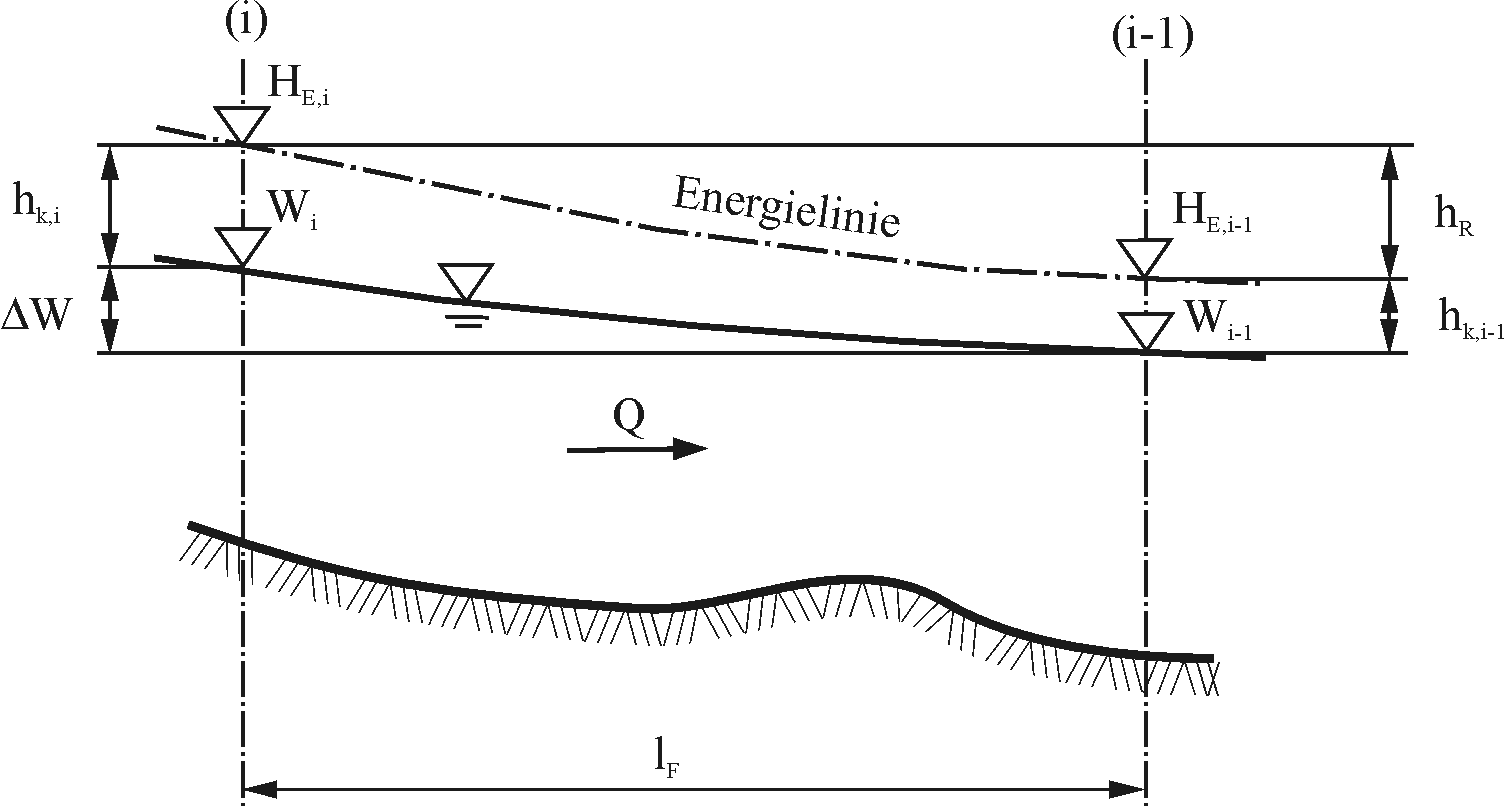
\includegraphics[scale=0.20]{Flussabschnitt}
   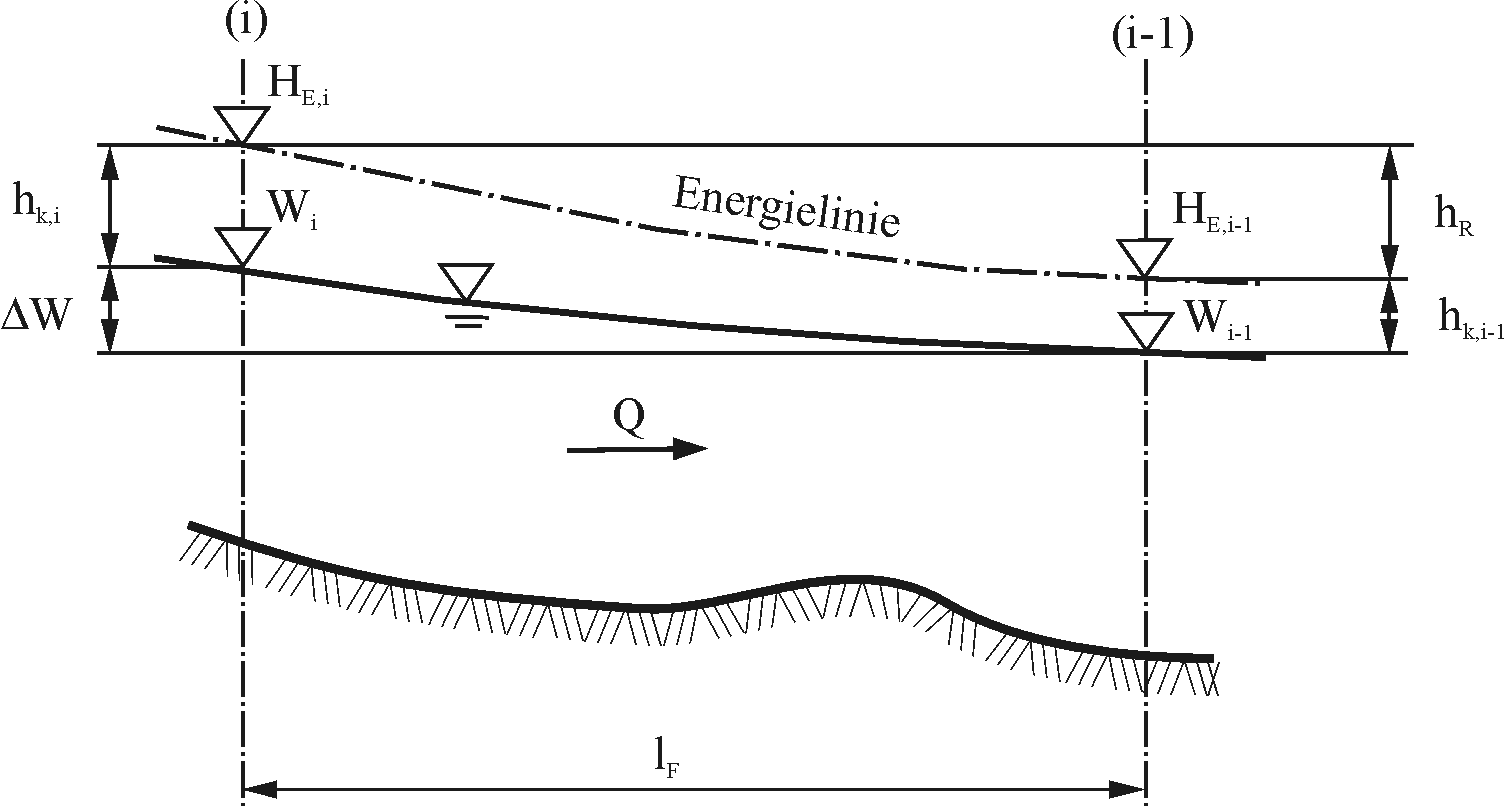
\includegraphics[width=0.8\linewidth]{Flussabschnitt}
   \caption{Flu{\ss}abschnitt $l_F$ mit Wasserspiegel und Energielinie}
   \label{Einfuehrung Abb Flussabschnitt}
\end{figure}
Mit den Bezeichnungen aus Abbildung~\ref{Einfuehrung Abb Flussabschnitt} ist
\begin{equation}
    W_i + h_{k,i}  =  W_{i-1} + h_{k,i-1} + h_R + H_{ZV}
\end{equation}
woraus sich durch einfache Umformung die Arbeitsgleichung ergibt:
\begin{equation}
    \Delta W  =  \Delta h_k + I_{E,m} \cdot l_F + H_{ZV}
\end{equation}
Hierbei bedeuten:
\begin{eqnarray*}
   \begin{tabular}{ll}
      $\Delta W = W_i - W_{i-1}$                               &  Differenz der Wasserst\"{a}nde \\
      $\Delta h_k = h_{k,i} - h_{k,i-1}$                       &  Differenz der Geschwindigkeitsh\"{o}hen \\
      $I_{E,m} = 0,5 \cdot (I_{E,i} + I_{E,i-1}) = h_R/l_F$    &  Mittleres Reibungsgef\"{a}lle \\
      $l_F$ 																									 & Profilabstand \\
      $H_{ZV}$                                                 &  Zus\"{a}tzliche \"{o}rtliche Verlusth\"{o}he
   \end{tabular}
\end{eqnarray*}
Die numerische L\"{o}sung dieser Gleichung erfolgt iterativ. Zun\"{a}chst wird aus dem Profilabstand und dem
Energieliniengef\"{a}lle des Profils~(i-1) der Wasserstandzuwachs $dh$ f\"{u}r das Profil~(i) gesch\"{a}tzt. F\"{u}r die sich dadurch
ergebende Wasserspiegelh\"{o}he $W_i = W_{i-1} + dh$ werden die erforderlichen geometrischen und hydraulischen Werte des
Profils~(i) berechnet. Mit dem daraus resultierenden Energieliniengef\"{a}lle $I_{E,i}$ kann die Verlusth\"{o}he ermittelt
werden, die zusammen mit der errechneten \"{A}nderung der Geschwindigkeitsh\"{o}he $dh_k$ eine neue Wasserspiegel\"{a}nderung $dW$
ergibt. Der Zuwachs $dh$ wird solange verbessert, bis sich dieser von dem errechneten Zuwachs $dW$ h\"{o}chstens um den
Wert der vereinbarten Genauigkeitsschranke $\mathit{EPSH}$ unterscheidet. In der Regel wird $\mathit{EPSH}$ zu
$0,005\unit{m}$ gew\"{a}hlt.

\subsection{Vorarbeiten}
Die zur Nachbildung der nat\"{u}rlichen Verh\"{a}ltnisse erforderlichen Vermessungsaufnahmen sollten bereits auf die
rechentechnischen M\"{o}glichkeiten des eingesetzten Wasserspiegellagenprogramms abgestimmt sein. Wenn eindimensionale
Rechenverfahren eingesetzt werden sollen, ist keine fl\"{a}chendeckende Gel\"{a}ndeaufnahme im Dezimeterbereich erforderlich, es
gen\"{u}gen Gel\"{a}nde-Querprofilaufnahmen in ausreichender Dichte.

Bei der Festlegung der Querprofile im Gel\"{a}nde ist den Besonderheiten, die sich aus der hydraulischen Problemstellung
ergeben, Rechnung zu tragen. Dies sind in erster Linie \"{U}berlegungen bez\"{u}glich des Querprofilabstandes, der Lage der
Profile im Lageplan, sowie der Ber\"{u}cksichtigung von Einbauten und sonstigen nat\"{u}rlichen Gegebenheiten wie z.B. Ufergeb\"{u}sch
oder Baumbewuchs. Wenn der Bewuchszustand einen merkbaren Einflu{\ss} auf das Str\"{o}mungsverhalten erwarten l\"{a}{\ss}t, so sind die
Buschgruppen und Baumreihen im Lageplan f\"{u}r eine Auswertung mit den entsprechenden Berechnungsverfahren mit aufzunehmen
(Abbildung~\ref{Einfuehrung Abb LageplanBewuchs}).

Bei Gerinneformen, die entsprechend einem Regelprofil ausgebaut worden sind, k�nnen gr��ere Profilabst�nde (l = 20 - 30 b) gew�hlt werden, bei sehr unregelm��iger Geometrie mit der M�glichkeit von schie�endem Abflu� k�nnen Profilabst�nde im Bereich der Gerinnebreite notwendig werden.
Grunds�tzlich sollte die Vermessung Querprofile in Flie�richtung gesehen liefern, d.h. in der Darstellung der Querprofile sollte das linke Vorland auch auf der linken Seite dar\-ge\-stellt sein.

\begin{figure}[hbt]
   \centering
   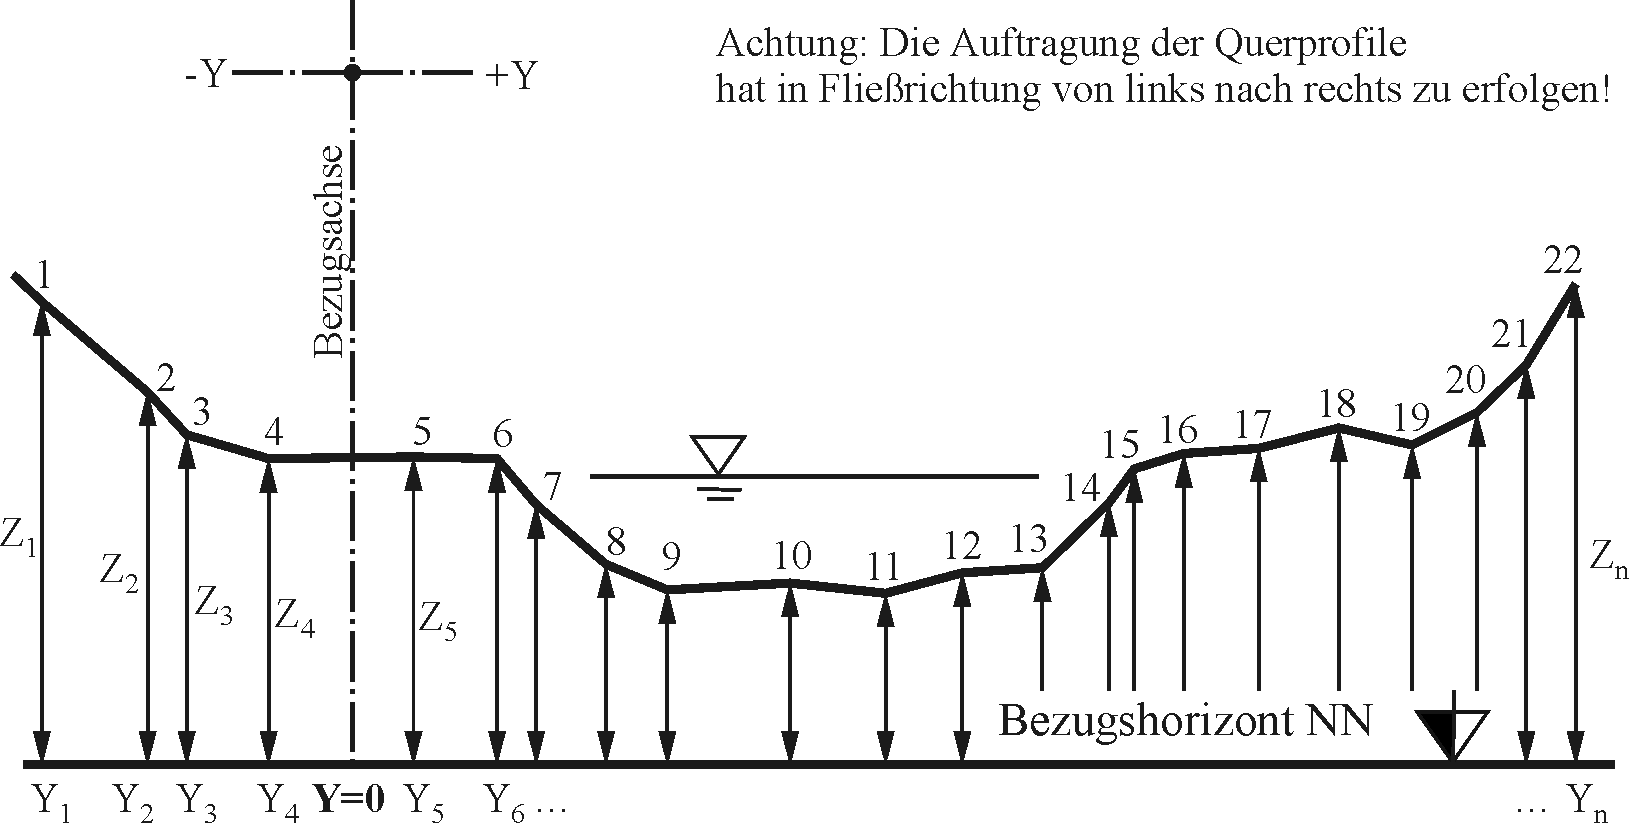
\includegraphics[width=0.8\linewidth]{ProfilaufnahmeKoordinaten}
   \caption{Beispiel einer Querprofilaufnahme (Eingabe in Koordinaten)}
   \label{Einfuehrung Abb Querprofilaufnahme}
\end{figure}
\begin{figure}[hbt]
   \centering
   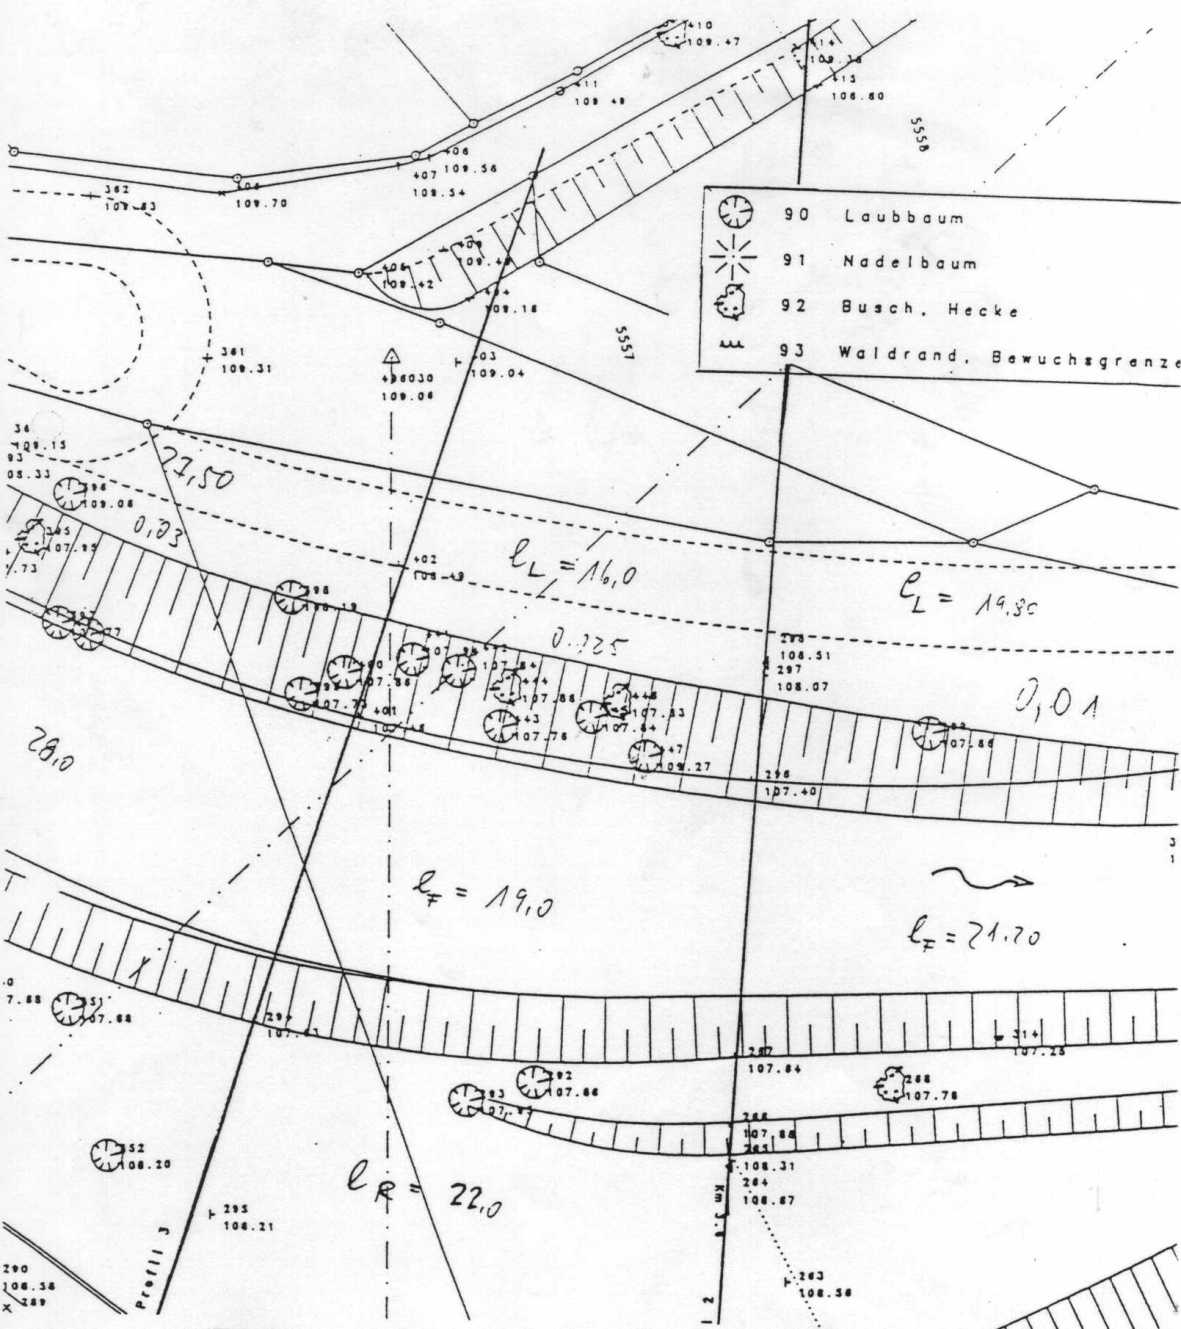
\includegraphics[width=0.8\linewidth]{LageplanBewuchs}
   \caption{Ausschnitt aus einem Lageplan mit eingezeichnetem Bewuchs}
   \label{Einfuehrung Abb LageplanBewuchs}
\end{figure}
Als Querprofildaten werden die Koordinaten des Profilpolygons ben\"{o}tigt:
\begin{itemize}
   \item horizontale Abst\"{a}nde der Profilpunkte ($y$-Werte) in $[\mathrm{m}]$ von einer beliebigen Bezugsachse
         (mit Vorzeichen einzugeben)
   \item H\"{o}he der Profilpunkte ($z$-Werte) in [$\mathrm{NN\!+\!m}$]
\end{itemize}
Liegen die Anfangs- bzw. Endpunkte des Profilpolygons unter dem berechneten Wasserspiegel, wird eine fiktive lotrechte
Begrenzung angenommen. Diese fiktive Begrenzung geht nicht in den benetzten Umfang ein, d.h. sie wird als reibungsfrei
betrachtet. Die Lage der Bezugsachse f\"{u}r die $y$-Werte ist beliebig. Es ist lediglich zu beachten, da{\ss} die Werte auf der
linken Seite der Achse ein negatives Vorzeichen haben m\"{u}ssen. Eine Variante f\"{u}r die Eingabe besteht darin, einen
Teilabflu{\ss}querschnitt des Flu{\ss}schlauchs in integraler Form einzugeben.

W\"{a}hrend f\"{u}r den Flu{\ss}schlauch der Abstand i.a. durch die Stationierung festgelegt ist, k\"{o}nnen bei den Vorlandteilfl\"{a}chen in
Flu{\ss}kr\"{u}mmungen hiervon abweichende Abst\"{a}nde auftreten. Aus diesem Grund ist es m\"{o}glich, die Abst\"{a}nde der Teilabflu{\ss}fl\"{a}chen
(linkes Vorland, Flu{\ss}schlauch, rechtes Vorland) getrennt einzugeben. Der Abstand wird dabei vom betrachteten
Profil~$(i-1)$ zum n\"{a}chsten oberstromigen Profil~$(i)$ gemessen. Als Abstand im Vorland kann die abgewickelte L\"{a}nge der
mittleren Strombahn des Vorlandteilabflusses betrachtet werden. Von besonderer Bedeutung ist hierbei, da{\ss} die
Abflu{\ss}verteilung in einem gegliederten Querschnitt von dem Verh\"{a}ltnis der Abst\"{a}nde zueinander abh\"{a}ngt. Ma{\ss}gebend f\"{u}r die
Abflu{\ss}verteilung im Querschnitt~$(i)$ sind die im Strang Profil~$(i-1)$ bis Profil~$(i)$ in der Strangtabelle angegebenen
Abst\"{a}nde.
